\subsection{Methods for Flat Features}
\label{sec:methods.flat}

% Author: Silvana

Flat features are features which are assumed to be independent of each other. 
No intrinsic or group-like structures are induced. 
For flat features, three different type of feature selection methods can be distinguished: 
\begin{itemize}
  \item Filter methods
  \item Wrapper methods
  \item Embedded methods
\end{itemize}
In this section, a short introduction on those three categories will be given, 
including a discussion of their benefits and disadvantages.

\subsubsection{Filter Methods}
\label{sec:methods.flat.filter}

% Author: Silvana

As the name suggests, filter methods try to filter out relevant features from
non-relevant ones. This is done by considering only the data set itself, while
the properties of the classifier used afterward are ignored.
 
This makes filter methods computationally efficient and somewhat flexible, 
as any classifier can be used on the filtered features.  

But this independence has also its drawbacks. As the characteristics of the 
specific classifiers are not considered, it is not known which one works 
best with the selected subset. Thus the selected subset does not guarantee optimal 
performance of the classifier.

because features are normally evaluated independent of each other, filter methods often
fail in removing redundant features. Some methods try to overcome this problem by 
considering possible correlations between features.

Filter methods perform two phases sequentially: First, they rank the features according 
to a certain metric. The features with the highest rankings are then chosen to train the
classifier. 

The following chapters will present some popular filter methods and the metrics they use
for ranking features.

\paragraph{Fisher Score}
\label{par:methods.flat.filter.fisher_score}

% Author: Silvana hat mal was rein getan

When using Fisher score as a criterion for feature selection, each feature is rated and selected independent of the others by calculating its individual fisher score. The intuition behind fisher score is to select features in a way so that in the resulting "feature space", data samples of the same class are close to each other, while the distances between data points of different classes are as big as possible. Algorithmically, this filter process is relatively easy to perform: after computing the fisher score for each feature, the features with the highest scores are selected. (How many features are chosen and the definition of when a score is high enough is an open choice and dependent on the application design.)

Despite its relative simplicity, this method has a major drawback. As no eventual correlation between the features is considered, it is likely that the optimal subset is not selected. For example, if two features score relatively low individually, they eventually would score high in combination and cause better classification results. For the same reason, fisher score cannot handle redundant features. When selecting two features, it is possible that the same accuracy in classification could be achieved with only one of them.

Generalized Fisher score (GFS) is an attempt to overcome this problem. Instead of evaluating one feature after the other individually, several features are considered simultaneously. GFS was tested and compared with other state-of-the art methods, including Fisher score, and proved to perform better in applications like face recognition and number recognition. For face recognition, GFS selected features (in this case pixels) with an asymmetric distribution over the whole face-area, while fisher score selected many pixels which where clustered in non-face areas. \cite{Gu:12}
  
\paragraph{Mutual information based}
\label{par:methods.flat.filter.mutual_information}

% Author: Flo - Silvana haut auch was rein
  
Mutual information is an approach to measure a variables dependency on
another variable. No mutual information means they are independent, high mutual
information means they are dependent on each other.

Some concrete algorithms that are based on this approach are:
\begin{itemize}
  \item Min redundancy max relevance
  \item Information gain
\end{itemize}

Min redundancy max relevance combines measures for redundancy and relevance, and
then selects features with high relevance and minimum redundancy.

Information gain measures the amount of information a feature provides when it
comes to class prediction. If a feature has good discriminative properties it is
chosen.


\paragraph{Relief}
\label{par:methods.flat.filter.relief}

% Author: Silvana
The original Relief-algorithm was presented by Kira and Rendell \cite{Kira:92}, and can be used for binary classification problems. The algorithm is efficient (it runs in polynomial time), robust and tolerant to noisy data, but the quality of the results depends on the number of iterations.
The basic idea is to use a weight vector, which has as many entries as there are features. In each iteration, an instance/variable x is chosen at random. Then the near-hit and near-miss instance of the remaining set in relation to x are selected: This is the most similar instance from the same class as x, and respectively the most similar instance of the different class. The euclidean distance between x and the near-hit and near-miss is calculated to determine if a feature is relevant or not.  

Intuitively, if a feature is relevant, the near-hits should be closer than the near-misses on average, while for irrelevant features, near-hits and near-misses are independent from each other. 
For each feature $f_i$, the corresponding weight $w_i$ in the weight-vector is updated dependent on those distances by applying equation \ref{relief}:

\begin{equation}
\label{relief}
w_i = - (x_i - nearhit)^2  + (x_i - nearmiss)^2
\end{equation}

Relevant features thus score values larger than zero, while irrelevant features become zero or negative. After a desired number of iterations, the features whose weights have a value above a certain threshold are chosen for the classification or further processing.

The original algorithm was further developed by \cite{Kononenko:97}. ReliefF  is extension so that the algorithm is able to handle incomplete data and multiple-class problems. 
RRELIEFF (Regressional ReliefF) \cite{Robnik-Sikonja:97} adapts the algorithm to handle also linear regression problems.

The family of Relief-algorithms and eventual adaptations have successfully been used on feature selection problems in the recent years. Moore used an adaptation called Tuned ReliefF (TuRF) for genetic analysis \cite{Moore:07}, where the worst features are removed systematically in each iteration. By removing a fixed number of features in each iteration, the accuracy of weight-estimation is increasing compared to the results of the original ReliefF algorithm. Eppstein and Haake \cite{Eppstein:08} criticize that for truly genome-wide association analysis, where a huge number of features is used (up to hundreds of thousands), all the proposed methods don't scale well and the estimated weights become basically random values. Very large scale ReliefF (VLSReliefF) tries to overcome this limitation by simply applying Relief on subsets of the features, and then combining the results to gain the weights for all features. This process can be parallelized on the GPU to speed it up \cite{Lee:15}

(Evtl. other application: One application was automated classification of websites \cite{Jin:07}.)


\subsubsection{Wrapper Methods}
\label{sec:methods.flat.wrapper}

% Author: Silvana

In contrast to filter methods, wrapper methods consider the properties of the classifier which will be used for classification.
The feature-set is selected so that it fits the biases and heuristics of the classifier as good as possible. 

Wrapper methods basically perform the following two steps iteratively: 

\begin{itemize}
  \item Search: A search routine selects a set of features 
  \item Evaluation: The selected subset is evaluated with the desired classifier
\end{itemize}

The search and evaluation steps are repeated until a stopping criterion is met, for example when a desired quality of classification is reached, 
or until a maximum number of iterations was performed. The subset which performed best is selected to train the actual classifier,
and normally, another evaluation with an independent testing set is done before actually using it for classification.
(See figure ~\ref{fig:methods.flat.wrapper.diagramm}) 

\begin{figure}[!ht]
  \centering 
  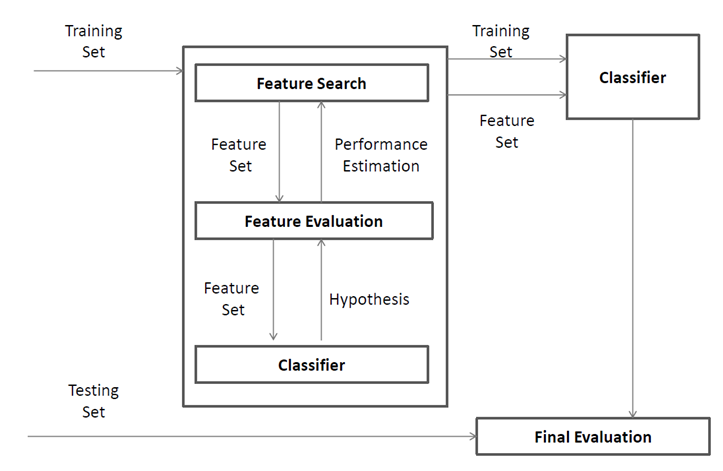
\includegraphics[width=0.8\textwidth]{chapters/methods/flat/wrapper_diagramm}
  \caption{Reprinted from \cite{Tang:14}. Basic scheme of a wrapper method. Using a training set, search and evaluation steps are performed iteratively.
	The search-algorithm provides potential feature-subsets which are evaluated by actually training the classifier. The quality is either heuristically estimated
	or evaluated by cross validation. After a stopping criterion is met, the actual classifier is trained and evaluated with an independent testing set again before
	being used for the actual classification task.}
  \label{fig:methods.flat.wrapper.diagramm}
\end{figure}

When choosing a search routine, the structure and size of the search space should be taken into account. As the feature space in the majority of 
applications is high dimensional, it is not possible to enumerate all possible feature subsets. Greedy algorithms are a popular choice,
but tend to get stuck in local optima when exploring big search spaces. in contrary, genetic algorithms are more complex, but are more likely
to explore the search space thoroughly and find a global optimum.

When a potential subset is found, its performance for the desired classifier has to be evaluated. 
This can be done for example by simply using a validation set, or by performing cross-validation.

The major drawback of wrapper methods is the computation time needed, as the subsequent search- and evaluation steps are computationally expensive: 
Every time a potential feature subset is selected, the classifier has actually to be trained with a training set and evaluated (for example by performing
cross validation, or using accuracy estimation.\cite{Kohavi:97}) Because the finally selected subset is dependent on the classification algorithm, 
it will eventually produce biased results when being used with an arbitrary classifier. 

Compared to filter methods, wrapper methods have the big advantage of selecting feature subsets which normally produce more accurate classification results.
Their better performance thus justifies the long computation time.

This next chapters will go more in-depth about the different search-techniques. First, the general strategies forward selection and backwards elimination 
are introduced, then search by greedy algorithms and genetic algorithms are explained in more detail.

\paragraph{Forward Selection/backward elimination}
\label{par:methods.flat.wrapper.forward_selection}

% Author: Silvana
In practice, two methods which are often used for large data sets are sequential forward selection (SFS) and sequential backward elimination (SBE).
 
Both  technique work  iteratively. Forward selection starts with an empty set, where no feature is selected in the beginning. 
Sequentially, one  feature after the other is added to the subset, so that the new subset maximizes the quality of  the  subset,
which is measured by some criterion function J. This is done until the set has reached a desired size. SBE works exactly the other way round, 
starting with the full set of features first and sequentially deleting features, until a smaller subset of sufficient quality is gained. 

Both methods have a major drawback: Either features cannot be eliminated once they have been selected (SFS), 
or they cannot be selected again if they have been discarded once (SBE). The assumption, that the best five selected features  must contain a 
subset of the best four selected features does not hold in practice. \cite{Nakariyakul:08}

\cite{Pudil:94} proposes Sequential forward floating selection as improvement (and, respectively, Selective backward floating elimination). 
A backtracking step is implemented after each sequential addition or deletion, which tries to find eventually better subsets. Both methods 
show admissible computation-time for small- or medium scaled problems, and perform better than other sequential methods on a variety of
problems. However, it should be empathized that they do not always perform better than other methods, but at least "good enough" on the 
majority of problems. For very big datasets, they are outperformed by genetic algorithms. \cite{Kudo:00}   

\cite{Mao:04} proposes \textit{orthogonal} forward selection and backward elimination to overcome problems that occur with SFS and SBE. 
Instead of simply selecting features in a sequential way, they are first mapped to an orthogonal space. 
This mapping decorrelates the features, so they can be evaluated and selected individually. 
After the selection, the features are linked back to the same number of variables in the original measurement space.
Using a mapping to orthogonal space proved to be very effective for features with high correlation. 
If the correlation between candidate features is only trivial, orthogonal
transforms don't improve the results compared to existing sequential methods.
\paragraph{Hill Climbing}
\label{par:methods.flat.wrapper.hill_climbing}

% Author: Silvana

Hill climbing, sometimes also referred to as "steepest ascend", is probably the simplest search technique that can be applied. Starting with no features at all, an evaluation function rates the available features and adds the most relevant one to the subset. Then the procedure is repeated, each time adding the most relevant feature of the remaining set to the subset. As soon as the influence of an added feature does not improve the overall quality of the set significantly, the search is stopped. The problem with hill climbing is that it gets stuck in local maxima easily, and fails in finding a globally optimal solution. \cite{Kohavi:97}

Best-first search outperforms hill-climbing and turns out to be a more robust technique according to Kohvani \cite{Kohavi:97}.
%\paragraph{Best First}
\label{par:methods.flat.wrapper.best_first}

% Author: Silvana
  
Best-first search outperforms hill-climbing, as it is a more robust technique. \cite{Kohavi:97} --Only one sentence and mentioned with hill climbing
\paragraph{Branch and Bound}
\label{par:methods.flat.wrapper.branch_and_bound}

% Author: Silvana

Branch-and-bound (BB) is a general design principle for solving discrete and combinatorial optimization problems. BB-algorithms work by building up a search tree with possible candidate solutions (branch phase). Further, a criterion function has to be designed, which evaluates the "quality" of possible solutions represented by nodes in the tree. Then, the branches of the tree are explored to find a global optimum for the given function. To avoid that the search is exploring the whole possible space, and thus degenerating to a brute-force-approach, it is limited by so-called bounds, which prune the tree when it becomes unlikely to find an optimum in the current branch. 

For feature selection, Narendra et al. \cite{Narendra:77} first proposed a BB-algorithm based on efficient subset selection. The root of the tree represents the full set of features, whereas leaf-nodes represent single features (or subsets of the smallest desired size). Monotonicity is required regarding the criterion function and the subsets. That means, if a current subset is below a bound, then its following child nodes are assumed to be also lower than that bound. Thus, the search in this particular branch can be aborted, and continued at another branch. Additionally, the sorting of the nodes is done with an efficient enumeration scheme to augment finding an optimal solution in a short amount of time.

The problem with BB-methods is that it is not guaranteed to perform better (faster) than exhaustive search methods. It is not granted that enough sub-trees will be pruned to speed up the search sufficiently, in worst-case, the criterion-function is evaluated for every node in the tree. Additionally, evaluating the function close to the root takes longer than evaluating it at the leaves. \cite{Somol:04} proposed a fast BB approach, which tries to keep the evaluations of the criterion function at a minimum to speed up the search. The algorithm is "learning" how the removal of features influences the functions value, and tries to "predict" changes without doing the actual computation. Only if the predicted value comes close to a bound, the criterion function is evaluated, otherwise the algorithm continues descending in the tree.

Adaptive branch and bound for feature selection \cite{Nakariyakul:07} also tries to reduce the number of evaluations of the criterion function, by applying several improvements. Already when building up the tree, the order of the nodes corresponds to the importance of the features. Then, instead of trying to descend sequentially from node to node, an adaptive, "jumping" search method is used to avoid more-or less redundant computations of the evaluation function. Additionally, the initial bound used in the search and also the initial search level are chosen in an optimal way. (Comment: only tested on 30 features?! Still check this out...)

\paragraph{Genetic Algorithms}
\label{par:methods.flat.wrapper.genetic}

% Author: Silvana

(SOURCE!!! basically written down by what Silvana knows from se bachelor thesis...)
Before explaining how GA can be used for for feature selection, 
a short introduction into the very basic concept of those algorithms has to be made. As the name implies, 
genetic algorithms are inspired by the way nature �works� in real life: parents carry specific genetic  information, 
and a (re-)combination of this information is passed to their kids in order to create �better� offspring from generation to generation. 
GA's imitate this behaviour by encoding the data they should work on or optimize in so-called chromosomes 
(which could be for examples vectors of numerical values). 
One is not limited to using numerical data, but this is a very common approach, 
as numerical values can be processed easily by the typical routines in a GA. 
A desired number of chromosomes is initialized at the beginning of the algorithm. 
They can be created randomly (f.ex by creating vectors with random values) or according to specific rules.
As the algorithm starts, different operations are applied to create new chromosomes: 
for example, a new chromosome can be obtained by combining the values of two already existing chromosomes, 
or by changing random values in an already existing chromosome. 

The resulting new chromosomes are then evaluated according to a fitness function, 
which basically measures how �good� a chromosome is suited for the underlying problem. 
The chromosomes then can be ranked, and the best ones are taken again to create new offspring. 
This procedure is repeated as long until a desired quality/result is achieved.

Just like branch and bound algorithms, GA are generally not suited for big feature spaces, 
as they try to explore the whole search space until a stopping criterion is met. 
This takes a lot of computation time when feature spaces are highly dimensional. 
The strength of GA is that they do not tend to get stuck at local optima 
(es for example Hill climbing algorithms do), but instead are likely to find global optima.

For feature selection, the chromosomes could correspond to subsets of the total feature set. 
The values in a chromosome would encode if a feature is selected or not. This can be achieved simply by using binary values: 
1 indicates that a feature is selected for a possible subset, and 0 indicates that it is not selected. 
Mutation and recombination operators would modify the chromosomes, 
and a fitness function would evaluate their quality for the underlying classifier 
(remember, each chromosome resembles a subset of features).

But one is not limited to binary values [XY] and [BLA] used GA to find optimal kernel setting for SVM. [quote those two papers found from  2006] 

  
TODO
Bla bla bla\ldots

\subsubsection{Embedded Methods}
\label{sec:methods.flat.embedded}

 % Author: Flo

TODO
Bla bla bla\ldots

http://crpit.com/confpapers/CRPITV113Huda.pdf 

As both filter and wrapper methods have different strengths and weaknesses, 
it seems only natural that research tried to combine both ideas to create so-called embedded methods, 
which are basically a hybrid of the former two. 
The strategy is to involve the classifier and its properties (like wrapper methods) while selection the features, 
and being computationally efficient at the same time (like filter methods).

Three types:

\begin{itemize}
  \item Linear Classifiers (Pruning methods, SVM, logistic regression)
  \item ID3 / C4.5 with build-in mechanism (WTF?) 
  \item Regularisation models
\end{itemize}

Regularisation models idea: fit the moddel, but try to have as many weightsas
possible small or close to 0, so we can eliminate features with small/zero weights


TODO:  more on embedded methods